% preamble with all definitions
\documentclass[12pt,letterpaper]{article}
\usepackage[utf8]{inputenc}
\usepackage[english]{babel}
\usepackage{amsmath}
\usepackage{amsfonts}
\usepackage{amssymb}
\usepackage{fancyvrb}
\usepackage{graphicx}
\usepackage[breaklinks=true]{hyperref}
\usepackage[hyphenbreaks]{breakurl}
\hypersetup{
       pdfauthor = {Kim Siang Khaw},
        colorlinks=true, citecolor=blue, linkcolor=blue, bookmarksnumbered = true,
}
\usepackage[left=2cm,right=2cm,top=2cm,bottom=2cm]{geometry}


\author{Renee Fatemi, Kim Siang Khaw, Liang Li, Adam Lyon}
\title{Data Production for the Muon g-2 experiment}
\begin{document}

\maketitle

\section{Production Workflow}
This document outlines the workflow of the data production of the Muon g-2 experiment. There are two different production chain: simulation and DAQ. 

\subsection{Simulation production workflow}
Simulation chain involves generating Geant4-based simulated data files, digitization of the truth information and reconstruction of the digitized information. Interaction between the gm2 instance and jobsub and SAM  in the simulation chain is summarized in Fig. \ref{fig:SimProd}.

\begin{figure}[htbp]
\centering
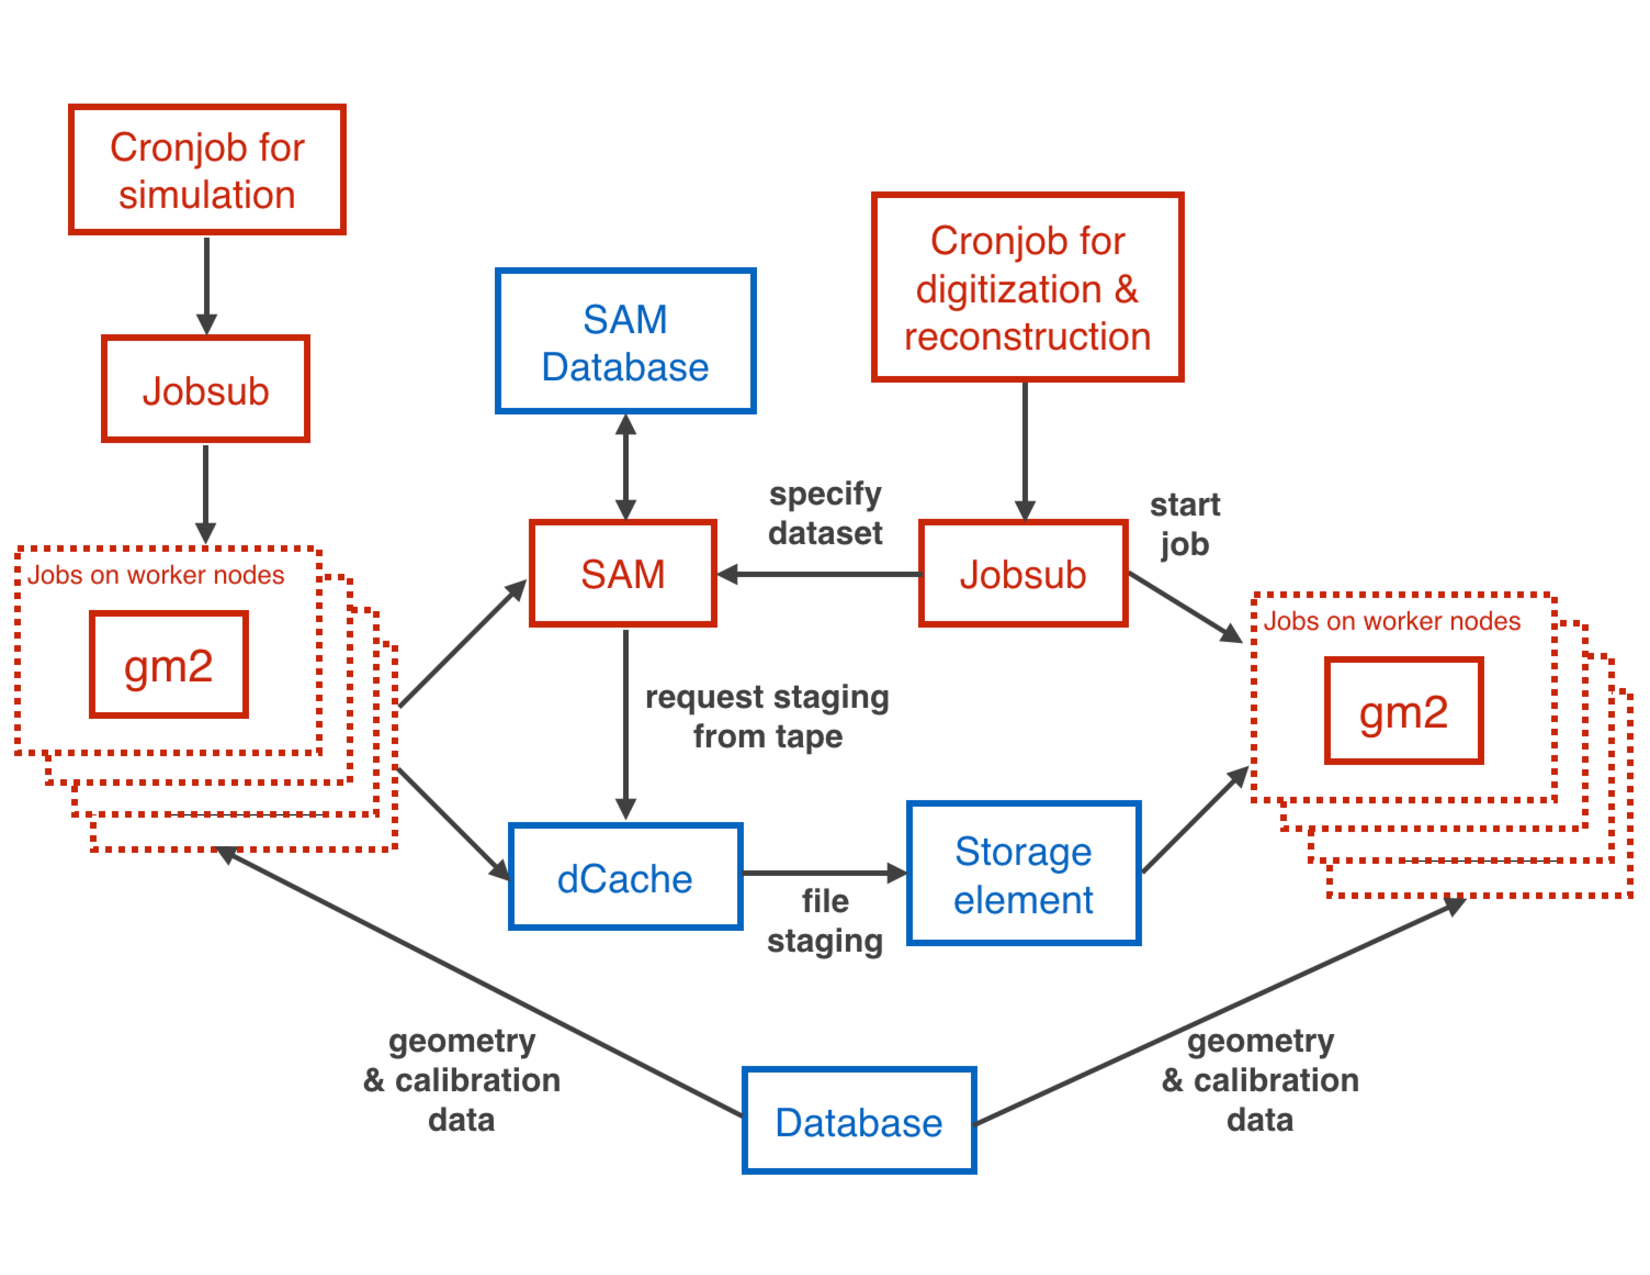
\includegraphics[width=0.7\textwidth]{pics/SimulationProductionWorkflow.pdf} 
\caption{Workflow for the simulation production.}\label{fig:SimProd}
\end{figure}

The following describes the basic steps in the simulation production:

\begin{enumerate}
\item A cronjob is setup to submit jobs to the FNAL grid at a specific time interval.
\item Worker nodes then execute the submitted scripts to generate simulated data. Database may or may not be used for the simulation.
\item Metadata of the generated data files are communicated to SAM data handling system and the files are transferred to FNAL permanent storage area.
\item Another cronjob independent of Cronjob1 is setup to submit jobs to the FNAL to digitize and reconstruct the simulated data.
\item Worker nodes then specify SAM dataset to be digitized and reconstructed.
\item The reconstructed data are then stored in the permanent storage area.
\end{enumerate}

\subsection{DAQ production workflow}

Interaction between the gm2 instance and jobsub and SAM in the DAQ chain is summarized in Fig. \ref{fig:DAQProd}.

\begin{figure}[htbp]
\centering
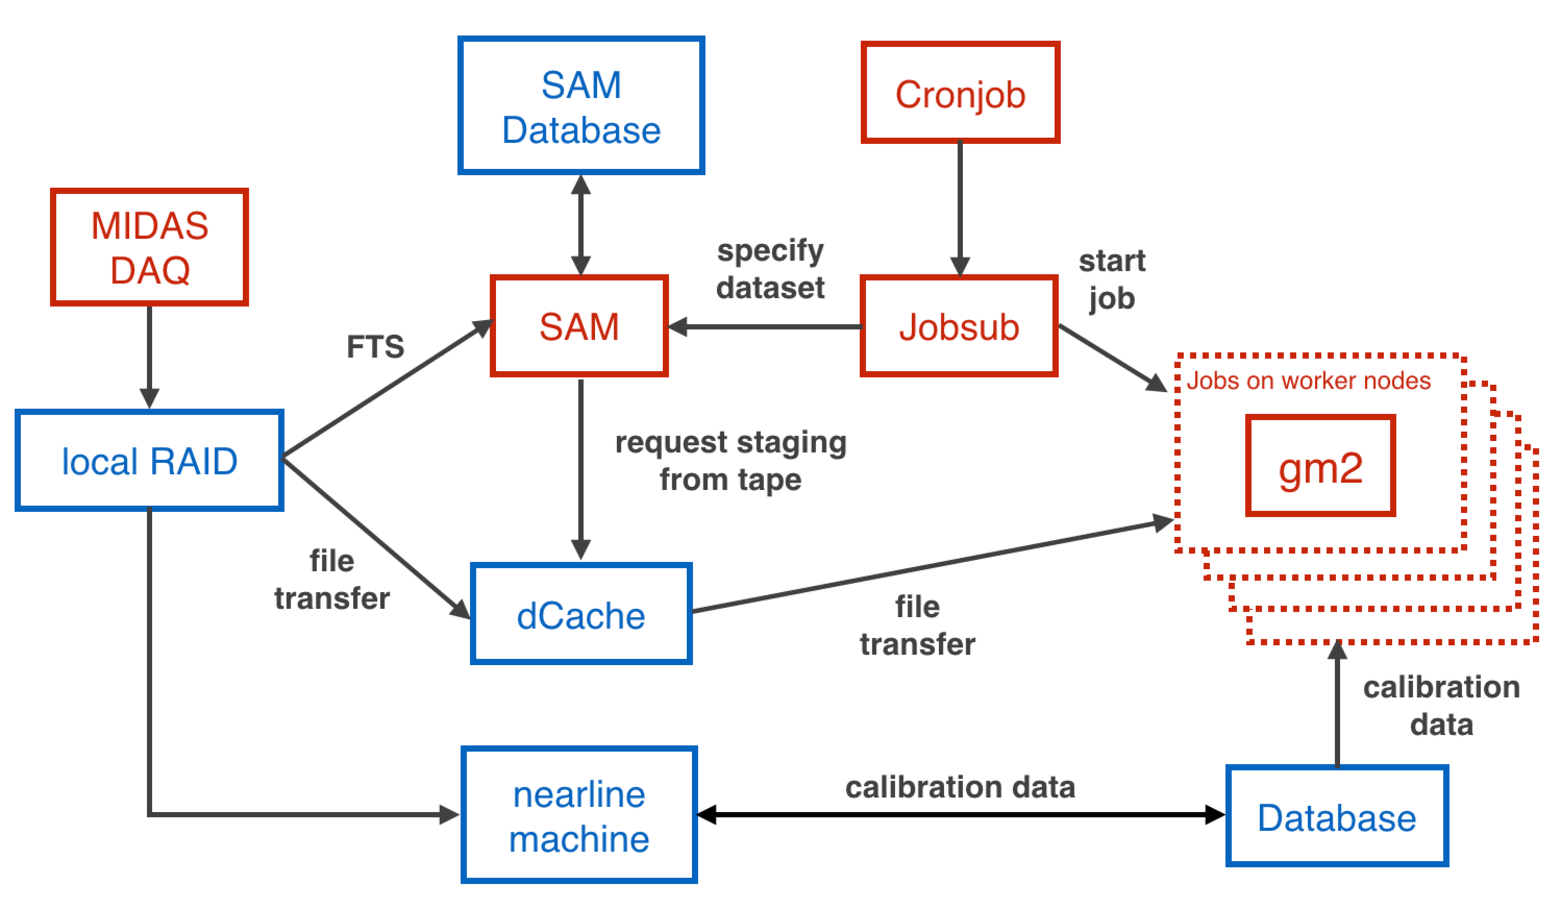
\includegraphics[width=0.7\textwidth]{pics/DAQProductionWorkflow.pdf} 
\caption{Workflow for the DAQ production.}\label{fig:DAQProd}
\end{figure}

The following describes the basic steps in the DAQ production:
\begin{enumerate}
\item MIDAS DAQ outputs raw data and stores them into local RAID storage.
\item A backend machine running FTS transfers raw files to the permanent storage area while communicates with SAM regarding the metadata of the files.
\item At the same time, a nearline machine analyzes specific calibration runs and extracts calibrations from these runs. All the constants are stored in the database.
\item A cronjob is setup to submit jobs to unpack and reconstruct the DAQ data.
\item Worker nodes then specify SAM dataset to be unpacked and reconstructed.
\item The reconstructed data are then stored in the permanent storage area.
\end{enumerate}

\section{SAM Metadata: Metadata definition and dataset definition}
How to insert metadata using FTS, art, etc. What are the metadata we want to insert, etc.

\section{Workflow of the data production: Implementation }

Once the production team is identified and assembled, the various types of production should be consolidated. The productions fall naturally into categories of simulation and real data, with the later divided into commissioning and runtime productions. 

\begin{itemize}

\item[I] Simulations
 \begin{itemize}
 	\item[i] MDC1 -  uses muon gas gun to produce sample of  $10^{10}$ muons (10$\%$ of muons  be collected in the experiment).
         \item[ii] MDC2 - uses inflector beam gun to produce sufficient sample size to develop lost muon analyses and study optimal  injection parameters for the kickers and quads. Detailed studies of beam dynamics and average spin effects will need much larger samples (TBD).
\end{itemize}

\item[II] Data
\begin{itemize}
 	\item[i]  Commissioning
		\begin{itemize}
		 \item[-] Mock Fast DAQ -  data taken with no detectors attached. Useful for Q-method studies.
		 \item[-] Laser - data taken in the months before beam arrives to test calorimeter, laser and DAQ system
		 \item[-] Magnetic Field DAQ - data taken during commissioning period to exercise DAQ
		 \item[-] Additional types to be identified ....
		 \end{itemize}
         \item[ii] Runtime
         \begin{itemize}
		 \item[-] FAST DAQ 
		 \item[-] Magnetic Field DAQ 		
		 \item[-] Fiber Harp
		 \item[-] Additional types to be identified ....
	\end{itemize}
\end{itemize}

\end{itemize}

\noindent Within these categories it will likely be necessary to make further distinctions, for example proton runs vs muon runs in the Runtime FAST DAQ category. This list will need to be worked out as the experiment progresses and updated here.\\

\noindent Of the productions listed above the MDC1 and Mock Fast DAQ are the most natural candidates to use for development and testing of the production workflow. The simulation framework in release $v7\_03$ is  production-ready and there are files on dCache from existing Mock Fast DAQ data.  If production tools were in place then job submission could commence immediately.  In  fact small productions, on the order of $\sim$ million events,  have already been produced for MDC1, and the entire SLAC test stand data has been produced.\\

\noindent In order to launch full scale productions the team needs to become proficient with the POMS tool, which will aid in tracking job submission.  The complete set of metadata needs to be defined for SAM (see Section 2 above) and submission scripts need to be written (see Section 4 below).  Eventually the team will also need to take advantage of the resources provided by the Open Science Grid, presumably this is the next step to take once production is running smoothly on FermiGrid.\\

\noindent Considering these tasks   the production team has set the goal of launching, in parallel, MDC1 and Mock DAQ data productions by February 1st.  The full production team is still being assembled and should be complete by the first week in December. The team will be composed of a Production Team Leader, Liang Li,  and four additional members, one which of which will serve as an onsite deputy leader.  The deputy leader, along with three other members will work with the leader to develop the POMS framework, SAM metadata and scripts. Half of the team will focus on the simulation productions (MDC1 to start) and the other half on the data productions (Mock DAQ).      

\section{Versioning of the scripts/codes (related to releases)}

\section{POMS: What do we know so far}
Reference slides:

\url{https://indico.fnal.gov/getFile.py/access?contribId=8&resId=0&materialId=slides&confId=12120}

\end{document}